\documentclass[paper=a4, fontsize=11pt]{scrartcl}
\usepackage[T1]{fontenc}
\usepackage{fourier}
\usepackage{listings}
\usepackage[english]{babel}															% English language/hyphenation
\usepackage[protrusion=true,expansion=true]{microtype}	
\usepackage{amsmath,amsfonts,amsthm} % Math packages
\usepackage[pdftex]{graphicx}	
\usepackage{url}
\usepackage{subcaption}
\usepackage{mathtools}
\usepackage{indentfirst}
\usepackage{color}
%%% Custom sectioning
\usepackage{sectsty}
\allsectionsfont{\centering \normalfont\scshape}


%%% Custom headers/footers (fancyhdr package)
\usepackage{fancyhdr}
\usepackage[utf8]{inputenc}
\pagestyle{fancyplain}
\fancyhead{}											% No page header
\fancyfoot[L]{}											% Empty 
\fancyfoot[C]{}											% Empty
\fancyfoot[R]{\thepage}									% Pagenumbering
\renewcommand{\headrulewidth}{0pt}			% Remove header underlines
\renewcommand{\footrulewidth}{0pt}				% Remove footer underlines
\setlength{\headheight}{13.6pt}



%%% Equation and float numbering
\numberwithin{equation}{section}		% Equationnumbering: section.eq#
\numberwithin{figure}{section}			% Figurenumbering: section.fig#
\numberwithin{table}{section}				% Tablenumbering: section.tab#


%%% Maketitle metadata
\newcommand{\horrule}[1]{\rule{\linewidth}{#1}} 	% Horizontal rule

\title{
		%\vspace{-1in} 	
		\usefont{OT1}{bch}{b}{n}
		\normalfont \normalsize \textsc{Instituto Superior Técnico} \\ [25pt]
		\horrule{0.5pt} \\[0.4cm]
		\huge Computação Móvel 2014/2015 \\
		\horrule{2pt} \\[0.5cm]
}
\subtitle{METI - TAGUS\\\small grupo 14}
\author{
  \normalsize Rui Pereira\\
  \normalsize \texttt{70600}\\
  \normalsize ruijosemangas@gmail.com\\
  \and
  \normalsize Pedro Braz\\
  \normalsize \texttt{73991}\\
  \normalsize pbraz.93@gmail.com
  \and
  \normalsize Patrícia Semedo\\
  \normalsize \texttt{79428}\\
  \normalsize patricia1990@live.com.pt\\
}

\date{}

%%% Begin document
\begin{document}
\maketitle
\newpage
\section{Objectivos Alcançados}

\begin{figure}[h!]
  \centering
    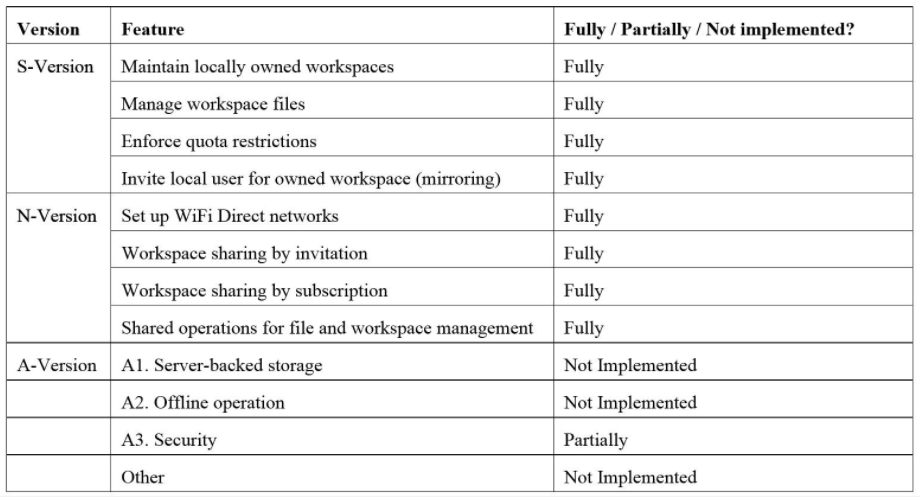
\includegraphics[width=1\textwidth]{images/table1.png}
\end{figure}

Em relação à parte avançada da implementação do projecto, desenvolvemos um mecanismo de segurança durante as escritas nos ficheiros. Este mecanismo permite que um utilizador, fazendo-se passar por outro, não consiga escrever no ficheiro.

\section{Especificações Técnicas}

\begin{figure}[h!]
  \centering
    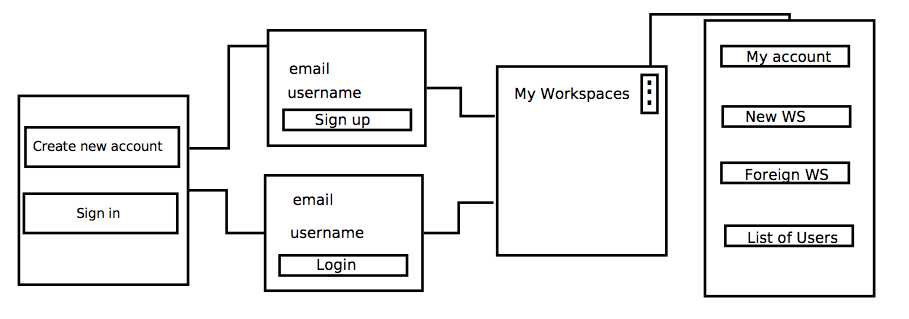
\includegraphics[width=0.9\textwidth]{images/cenas1.png}
\end{figure}

\begin{figure}[h!]
  \centering
    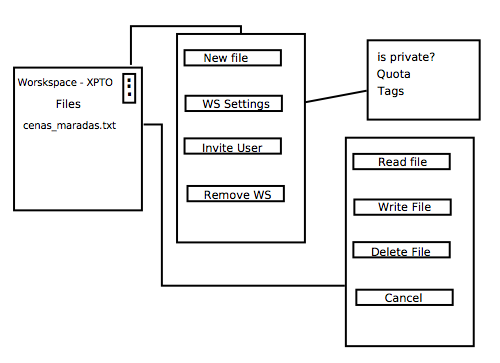
\includegraphics[width=0.7\textwidth]{images/ola.png}
\end{figure}

\newpage
\section{Desenho da Aplicação}

\subsection{Plataforma escolhida}
O projecto, foi desenvolvido e testado para correr em dispositos reais pois correr o projecto em simuladores é uma tarefa muito intensiva.
\subsection{Arquitectura}
Todo o estado da aplicação, é guardado de forma persistente numa base de dados relacional \textit{SQLite}. Os ficheiros são guardados internamente no dispositivo móvel. A aplicação funciona de maneira distribuída usando o \textit{Wi-Fi Direct} com o objectivo de haver partilha de informação entre diversos utilizadores na mesma rede. Na camada superior ao \textit{Wi-Fi Direct} é corrido um servidor que aceita vários pedidos em simultâneo.
\subsection{Protocolos utilizados}
Quando um utilizador entra na aplicação, liga-se a outros utilizadores que já estejam a usar a aplicação na tentativa de formar um grupo dentro da rede. Se o grupo já estiver formado, o novo utilizador contacta o \textit{group owner} para obter informação acerca de todos os utilizadores do grupo. Na rede, os utilizadores partilham os nomes dos \textit{workspaces} que possuem com todos os utilizadores do grupo.

Em relação ao \textit{subscribe}, o utilizador tem duas opcções: subscrever a todos os \textit{workspaces} públicos fornecendo uma \textit{query} vazia ou procurar por \textit{workspaces} específicos com base em \textit{tags}. O utilizador guarda o nome do \textit{workspace} na sua base de dados. Se o dono do \textit{workspace} estiver no grupo, ele pode aceder aos ficheiros. Se o dono apagar o \textit{workspace}, esse deixa de ser propagado na rede e quem o tiver subscrito sabe que o \textit{workspace} foi apagado.

Quando um \textit{user} quer aceder a ficheiros dentro de um \textit{workspace} remoto, é feito um pedido em \textit{real time} ao dono do mesmo. Este responde com os nomes dos ficheiros disponíveis e a \textit{view} da aplicação do utilizador inicial é actualizada. Todos este pedidos são feitos em \textit{background} na camada do servidor. Se um utilizador desejar aceder ao conteúdo de um ficheiro, é feito um pedido com a intenção do utilizador. Em ambos os casos(ler ou escrever), é necessária uma leitura da versão mais recente do ficheiro. A diferença é que se o utilizador quiser escrever, é criada uma sessão que impede escritas em simultâneo. Esta sessão termina quando o utilizador que escreve aceita ou cancela as alterações de escrita.

A sessão referida anteriormente, é bloqueada pelo dono do ficheiro que entrega uma chave ao utilizador para ser devolvida quando as alterações terminarem. Se a chave for a mesma que o dono entregou inicialmente, quer dizer que foi o \textit{user} correto a submeter as alterações. Após esta verificação, o dono faz \textit{commit} ao ficheiro.

Tentámos minimizar a latência na rede diminuindo a quantidade de informação que é transmida. Os ficheiros são transferidos \textit{on demand}.
\section{Implementação}
\section{Conclusão}
Em suma, o nosso projecto tem margem para algumas melhorias. Em relação às partes avançadas começamos a implementar a parte da segurança contudo ficou inacabada. Queríamos ter desenvolvido um protocolo mais coeso que fornecesse uma maior segurança dos dados trocados na rede. Para trabalho futuro podíamos desenvolver as outras componentes avançadas do projecto e uma interface gráfica melhor.

Em relação à componente prática da cadeira julgamos que o \textit{Wi-Fi direct} devia ser introduzido mais cedo. Além disso o código desenvolvido na primeira parte do projecto foi muito alterado para conseguir suportar a componente distribuída. Na nossa opinão a segunda parte devia ser a implementação de um novo módulo que não entrasse em conflito com a primeira parte. 
\end{document}